\section{Architecture}
\subsection{Overview}
Jetpack Compose is based on the concept that the View recompose(redraws) itself according to the changes in data state. Therefore the Data/Model we provide to the View has to be wrapped in Mutable States, a Jetpack Compose object which is observed by Compose, which means the View is updated automatically on data change.

With larger applications, a lot of stateful data has to be maintained and updated to keep the View in sync. The data must also be managed and updated correctly to trigger the recompose. For example: changing an item in a list which is wrapped in a Mutable State may not trigger a recompose.

\begin{kotlincode}
var tabs = mutableStateListOf(Tab(1, "Tab1"), Tab(2, "Tab2"))

fun changeTabName1(id: Int, newName: String) {
    tabs.first { it.id == id }?.name = newName
}
\end{kotlincode}

In the example above, you cannot simply change a tab in the list to generate a recompose. Instead, the state only refers to the list. The list must therefore be changed, e.g. by removing the tab to be changed and inserting it again.

\begin{kotlincode}
fun changeTabName(id: Int, newName: String) {
    tabs.removeIf { it.id == id }
    tabs.add(Tab(id, newName))
}
\end{kotlincode}

With an increased number of Mutable States it becomes more complex to maintain an overview of the recomposes triggered with each change. One Recompose can lead to data changes which then in turn trigger other recomposes. The worst case scenario is an infinite recompose loop which impacts the whole application.

To address these problems, we have chosen the approach of the single immutable state. To achieve this an instance of a data class is passed to the view as one state. All members of the class, which are the actual data, are immutable.

\begin{center}
    \begin{figure}[H]
            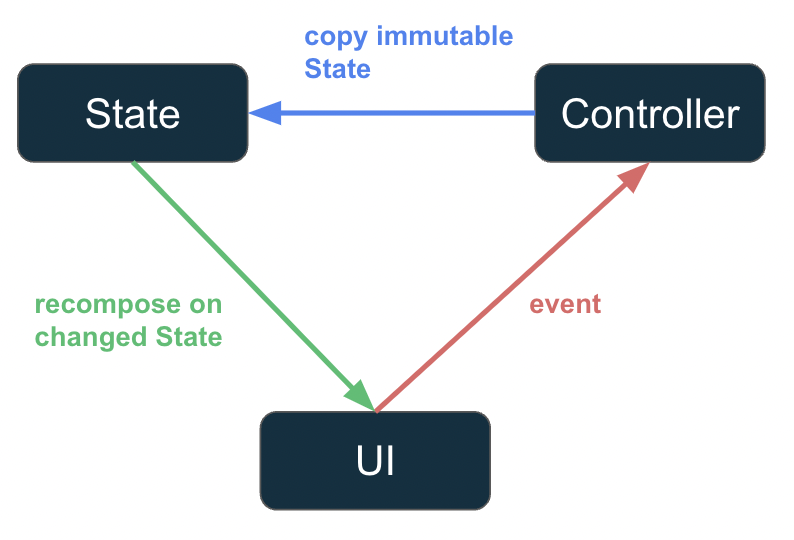
\includegraphics[width=0.6\textwidth]{images/unidirectional data flow.png}
            \centering
            \caption{Unidirectional data flow}
   \end{figure}
\end{center} 

An event from the UI that is to change the data is accepted by the controller. There, a new instance of the data class is created by copying and returned to the view as a new state.
With copy, the members to be changed can be specified as arguments, which allows efficient copying of objects in Kotlin.

This way the recompose is bundled to one point and view, controller and state are cleanly separated. In addition, concurrent changes of state are much easier to handle as they can only be made in one place.


\section{Class Diagram}
\begin{center}
    \begin{figure}[H]
            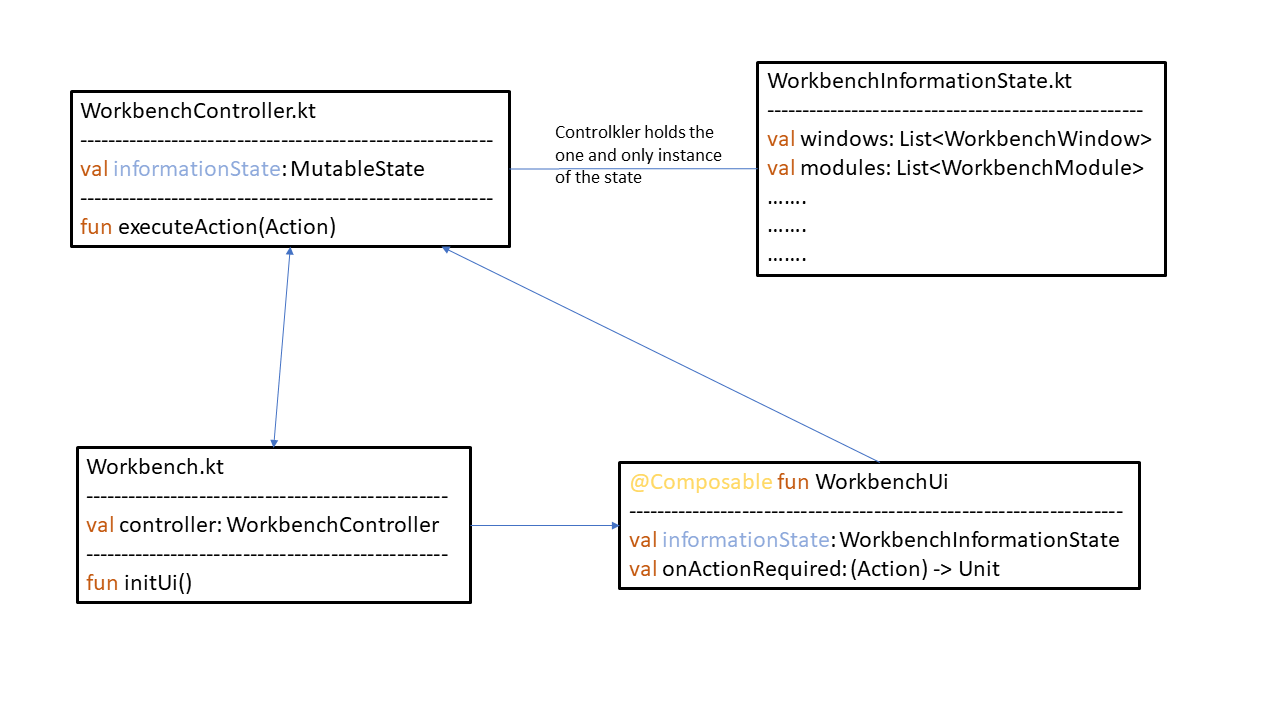
\includegraphics[width=0.8\textwidth]{images/classDiagram.png}
            \centering
            \caption{Simplified classdiagram}
   \end{figure}
\end{center} 

This Simplified class diagram shows the main classes and how they interact.
\begin{itemize}
    \item WorkbenchInformationState: A immutable data class which holds state relevant for the view
    \item WorkbenchController: Holds the only instance of the state as a Mutable State and provides one entry point (executeAction) to manipulate the state
    \item Workbench: The main class which initializes the controller and the view
    \item WorkbenchUi: @Composable function which is the entry point for the Ui
\end{itemize}

The WorkbenchUi receives the state and a callback to execute actions on the controller but not the controller itself to ensure it can only ever call this function. Once executeAction is called the Mutable State in the controller is updated which will trigger a recompose of the WorkbenchUi


\section{Messaging System}
To prevent the exchange of Code from the Workbench and integrated custom Modules or even between custom Modules, but still allow an interaction between those, a Messaging System is provided by the Workbench. 

For the Messaging System an embedded Version of a MQTT Broker is initialized within the Workbench. (https://github.com/hivemq/hivemq-community-edition)
The Address and Port of this Broker are not yet public and cannot be configured by the User. To keep the Messaging System Workbench "internal", a Workbench MqClient is initialized by the Workbench and exposed on certain interfaces, when registering or requesting Workbench Modules.

It is possible to publish (send Messages) and subscribe (receive Messages) to any topic. These actions are called asynchronous and for the subscribe a callback has to be defined to handle receiving messages.

\subsubsection{Topics}

Topics in MQTT are Strings, which are compared to each other to decide if a Client did subscribe for it. To organize Topics MQTT uses / as Sperator, and also offers also Wildcards.
\begin{figure}[H]
\centering
\begin{subfigure}{.5\textwidth}
  \centering
  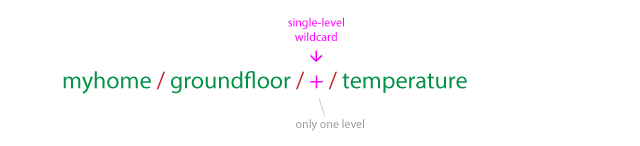
\includegraphics[width=.9\linewidth]{images/topic_wildcard_plus.png}
\end{subfigure}%
\begin{subfigure}{.5\textwidth}
  \centering
  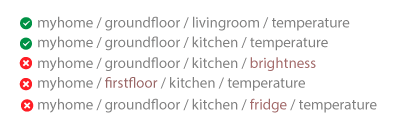
\includegraphics[width=.9\linewidth]{images/topic_wildcard_plus_example.png}
\end{subfigure}
\caption{Wildcard + to access a single level \citep{HiveMQ:MQTT-Essentials}}
\end{figure}

\begin{figure}[H]
\centering
\begin{subfigure}{.5\textwidth}
  \centering
  
\includegraphics[width=.9\linewidth]{images/topic_wildcard_hash.png}
\end{subfigure}%
\begin{subfigure}{.5\textwidth}
  \centering
  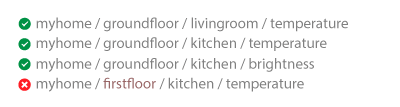
\includegraphics[width=.9\linewidth]{images/topic_wildcard_hash_example.png}
\end{subfigure}
\caption{Wildcard \# to access multi level \citep{HiveMQ:MQTT-Essentials}}
\end{figure}

So it's best practice to use the topics like a REST API, to take full advantage of these features.

For example if you want to publish a change of a Data field of the type City in our CityApp.
\begin{kotlincode}
mqClient.publish("city-app/city/$id/$field", value)
\end{kotlincode}

and on the other side to subscribe to any changes on a City.
\begin{kotlincode}
mqClient.subscribe("city-app/city/#", ::updateTempChanges)
\end{kotlincode}


\section{Asynchronous actions execution}
To prevent blocking the main thread where the UI is running, on executing resource and time consuming actions, it's important to run actions asynchronous. To handle actions asynchronous they have to be queued and must keep their order of execution. For this kind of use Kotlin offers channels. 
On a channel, information (Objects) can be shared between coroutines, by send to and receive from a channel.

A channel provides multiple options for how information is queued and processed. In our case we're using a unlimited buffered channel. Unlimited means that the send is never suspended until the application would run out of memory.
We assume this will not happen, because a Workbench has only few actions being called and most of them can be executed fast.

\begin{center}
    \begin{figure}[H]
            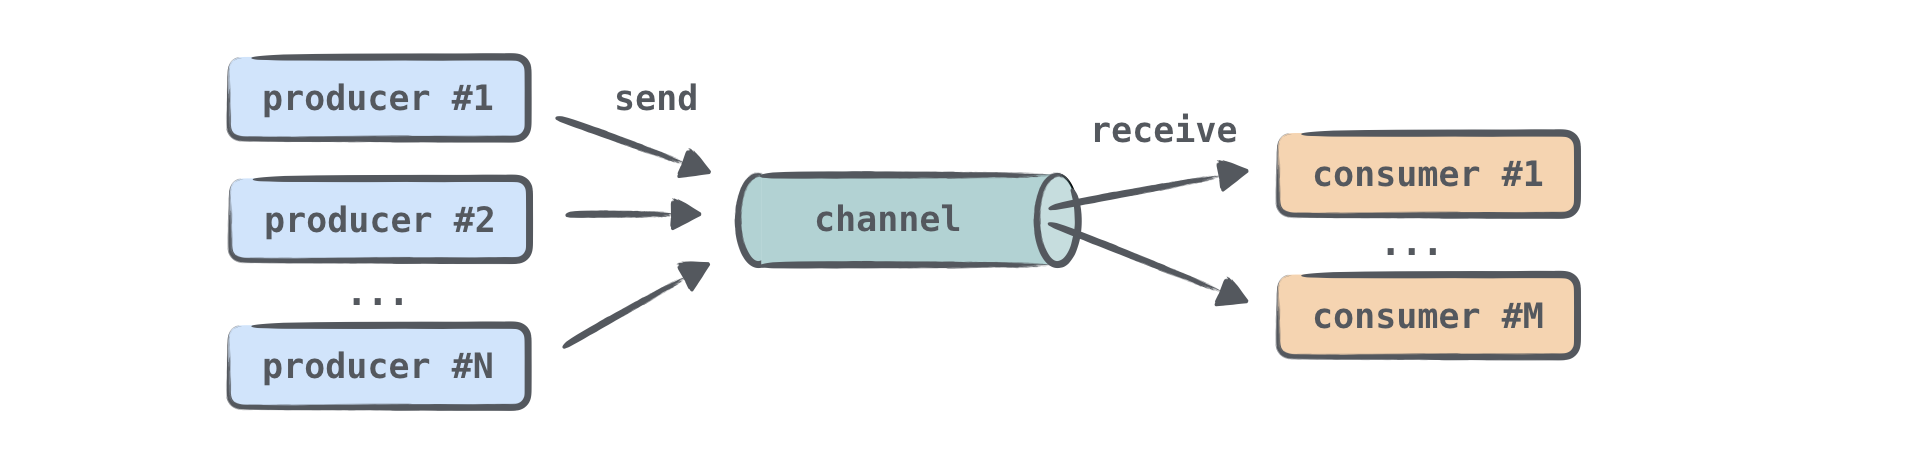
\includegraphics[width=0.7\textwidth]{images/UsingChannelManyCoroutines.png}
            \centering
            \caption{Channel concept in Kotlin \citep{KotlinLang:Playground}}
   \end{figure}
\end{center} 

To guarantee a deterministic behavior of the Controller and its state only one coroutine is receiving actions from the channel and make changes of the state. There would be actors to ensure only one coroutine is receiving message of the channel. But Actor of coroutines are  obsolete, so we skipped using it. 
On the other side any amount of coroutines are allowed to send actions to the channel.

\subsection{Synchronous actions}
Some of the actions have to be executed synchronous, otherwise the correct behavior of the Workbench is not guaranteed. For example a registration of a Module must be synchronous. Otherwise if a request is called before the registration is completed we can't request these kind Modules. 

For the synchronous action a class is introduced which hold a CompletableDeferred as response.

\begin{kotlincode}
internal sealed class WorkbenchActionSync(
    name: String,
    val response: CompletableDeferred<Int> = CompletableDeferred()
): WorkbenchAction(name) 
\end{kotlincode}

The action trigger is waiting for the response to be completed. Because the triggerAction is runBlocking it's caller is blocked until the response is set completed by the actionChannel consumer.

\begin{kotlincode}
private fun triggerAction(action: Action) = runBlocking {
    launch {
        actionChannel.send(action)
    }
    if (action is WorkbenchActionSync) {
        action.response.await()
    }
}
\end{kotlincode}


\section{Trailing lambdas} \label{Traling_lambdas}

According to Kotlin convention, if the last parameter of a function is a function, then a lambda expression passed as the corresponding argument can be placed outside the parentheses \citep{KotlinLang:TrailingLambdas}

This language feature is heavily used throughout Jetpack Compose. For example in UI elements such as columns and rows where the last argument of the Column() function is the actual content of the Column. This allows function calls which look and feel more like functions itself

\begin{kotlincode}
Column {
    Card ( onClick = { println("clicked")}) {
        Text(text = "click me")
    }
}
\end{kotlincode}

In this example, the Card with its text and onClick action is an Argument to the Column function.

In order to make the Workbench consistent with Jetpack Compose and to ensure a easy to use handling the Workbench is also making heavy use of trailing Lambda functions. Trailing Lambdas are used so the user can define the Content of the Modules when registering them. Interaction with the Workbench is done solely using functions.